%----Rules for writing with Geoff
% 1. No second person, unless you are serious saying "this is what __we__ did. Rather use third
% person passive, e.g., instead of "we did this" use "this was done".
% 2. Start each sentence on a new line, to make it easy to reorder sentences.
% 3. Send me your BibTeX entries - I'll add them to the bibliography file in my standard format.
%----
\documentclass[runningheads]{llncs}

\usepackage[T1]{fontenc}
\usepackage{graphicx}
% \renewcommand\UrlFont{\color{blue}\rmfamily}
\usepackage{hyperref}
\usepackage{color}
\usepackage{setspace}
\usepackage{verbatim}
\usepackage{multicol}
\usepackage{array}
\usepackage{bbding}
\usepackage{enumitem}

%----Making things more compact
%----Suppress extra space in texttt mode
%\AddToHook{cmd/ttfamily/after}{\frenchspacing}
\renewcommand{\textfraction}{0.07}
\renewcommand{\topfraction}{0.9}
\renewcommand{\bottomfraction}{0.9}
\renewcommand{\floatpagefraction}{0.66}
\setlength{\tabcolsep}{3pt}
\setlength{\floatsep}{2.0pt plus 2.0pt minus 2.0pt}
\setlength{\textfloatsep}{5.0pt plus 2.0pt minus 0.0pt}
\renewcommand{\textfloatsep}{2.0ex}
\renewcommand{\dbltextfloatsep}{2.0ex}

\newcommand{\proves}{{\footnotesize {\raisebox{0.3ex}{$\;\models$\;}}}}
\newcommand{\smalltt}[1]{\small \texttt{#1}}
\newcommand{\mytilde}{\raisebox{0.4ex}{\texttildelow}}
\newenvironment{packed_itemize}{
\vspace*{-0.2em}
\begin{itemize}
\setlength{\partopsep}{0pt}
\setlength{\itemsep}{1pt}
\setlength{\parskip}{0pt}
\setlength{\parsep}{0pt}
}{\end{itemize}}
\newenvironment{packed_enumerate}{
\vspace*{-0.2em}
\begin{enumerate}
\setlength{\partopsep}{0pt}
\setlength{\itemsep}{1pt}
\setlength{\parskip}{0pt}
\setlength{\parsep}{0pt}
}{\end{enumerate}}

\begin{document}

\title{The TPTP Format for Tableaux Proofs}
\titlerunning{TPTP Tableaux}

\author{
Geoff Sutcliffe\inst{1}\orcidID{0000-0001-9120-3927}\Envelope
\and
\\ Sean B. Holden\inst{2}\orcidID{0000-0001-7979-1148}
\and
\\ Mantas Baksys\inst{2}\orcidID{0000-0001-9532-1007}
}
\authorrunning{Geoff Sutcliffe, et al.}
\institute{University of Miami, USA,
\email{geoff@cs.miami.edu},
\and
University of Cambridge, United Kingdom,
\email{sbh11@cl.cam.ac.uk,mb2412@cam.ac.uk}
}

\maketitle
%--------------------------------------------------------------------------------------------------
\begin{abstract}
This paper describes the (new) TPTP format for recording tableau proofs.
The format builds on the existing infrastructure of the TPTP World, in particular the TPTP format
for recording derivations.
An ATP system that outputs tableau in this format is described.
Existing TPTP World tools for verifying and viewing derivations can be directly extended to
verify and view tableau proofs recorded in this new format.
\keywords{TPTP, tableau, proof}
\end{abstract}
%--------------------------------------------------------------------------------------------------
\section{Introduction}
\label{Introduction}

Automated Theorem Proving (ATP)~\cite{RV01-HAR} is concerned with the development and use of 
software that automates sound reasoning: the derivation of conclusions that follow inevitably 
from known facts.
ATP is at the heart of many computational tasks, including sensitive tasks such as 
software/hardware verification~\cite{HH19} and system security~\cite{Coo18}.
% New and emerging application areas include
% chemistry \cite{Yad17}, 
% biology \cite{CC+13}, 
% medicine \cite{HLB05},
% elections \cite{Nip09,BDS17}, 
% auctions \cite{CK+15}, 
% privacy \cite{Lib20},
% law \cite{PS15}, 
% ethics \cite{DF+16}, 
% religion \cite{OZ11,BW14-ECAI,Hor19},
% and business \cite{Han98}.
ATP systems are often used as components of more complex Artificial Intelligence (AI) systems,
which means that the impact of ATP extends into many facets of society.
% in areas such as 
% knowledge representation \cite{TR+04}, 
% natural language processing \cite{BM05}, 
% planning \cite{NV07}, 
% agents \cite{TBP03}, 
% commonsense reasoning \cite{MS05}, 
% and the semantic web \cite{McG04}.
In many of these applications the use of ATP systems is mission critical, in the sense that 
incorrect results from ATP might have nasty consequences.
% The importance of verifying the results from autonomous systems (including ATP systems) is
% reflected in the IEEE~P2817 standard, which aims to ``identify best practices and provide guidance 
% that supports the definition of valid verification processes for a range of autonomous system 
% configurations''.\footnote{%
% \href{https://standards.ieee.org/ieee/2817/11726/}{\smalltt standards.ieee.org/ieee/2817/11726/}}
Facing the demand for error-free results from ATP systems is the reality that ATP systems
are complex pieces of software, implementing complex calculi with complex data structures and
algorithms~\cite{Sch06}. 
Despite best intentions and efforts, incorrect results are possible.
% Two forms of incorrectness are most evident. 
% Firstly, an ATP system claiming to have found a solution when there is none, e.g., claiming to 
% have proved a non-theorem.
%MODEL or established the consistency of an unsatisfiable set of formulae. 
% Secondly, outputting a flawed solution, e.g., a proof that contains unsound inferences.
%MODEL or a model that has contradictory mappings for the symbols in the input problem.
To counter incorrectness, an ATP system can be required to output a proof
%MODEL solution, e.g., a proof or a model, which 
that serves as a certificate for the system's claim.
To ensure that a 
%MODEL solution 
proof is correct, proof verification can be required, 
which serves as a certification (but not a certificate) of the proof.
%MODEL solution.
% If the verifier outputs evidence for the certification in a form that can be independently 
% checked, that evidence serves as a certificate for the verifier's claim.
% As a concrete example, consider the verification process for aerospace software, shown in 
% Figure~\ref{NASACodeCertification}, taken from ~\cite{SDF05}.
% The ``proofs'' output by the ATP system are certificates that the ``safety policy'' has been 
% verified.  
% However, certification authorities like the FAA must be given explicit evidence that 
% the individual tool components (here, the ``ATP'' system) yield correct results.
% To that end the ATP system's proofs are given to a ``proof checker'' that produces certificates 
% that are attached to the ``code''.
%  
% \begin{figure}[htb]
% \begin{center}
% %EASYCHAIR 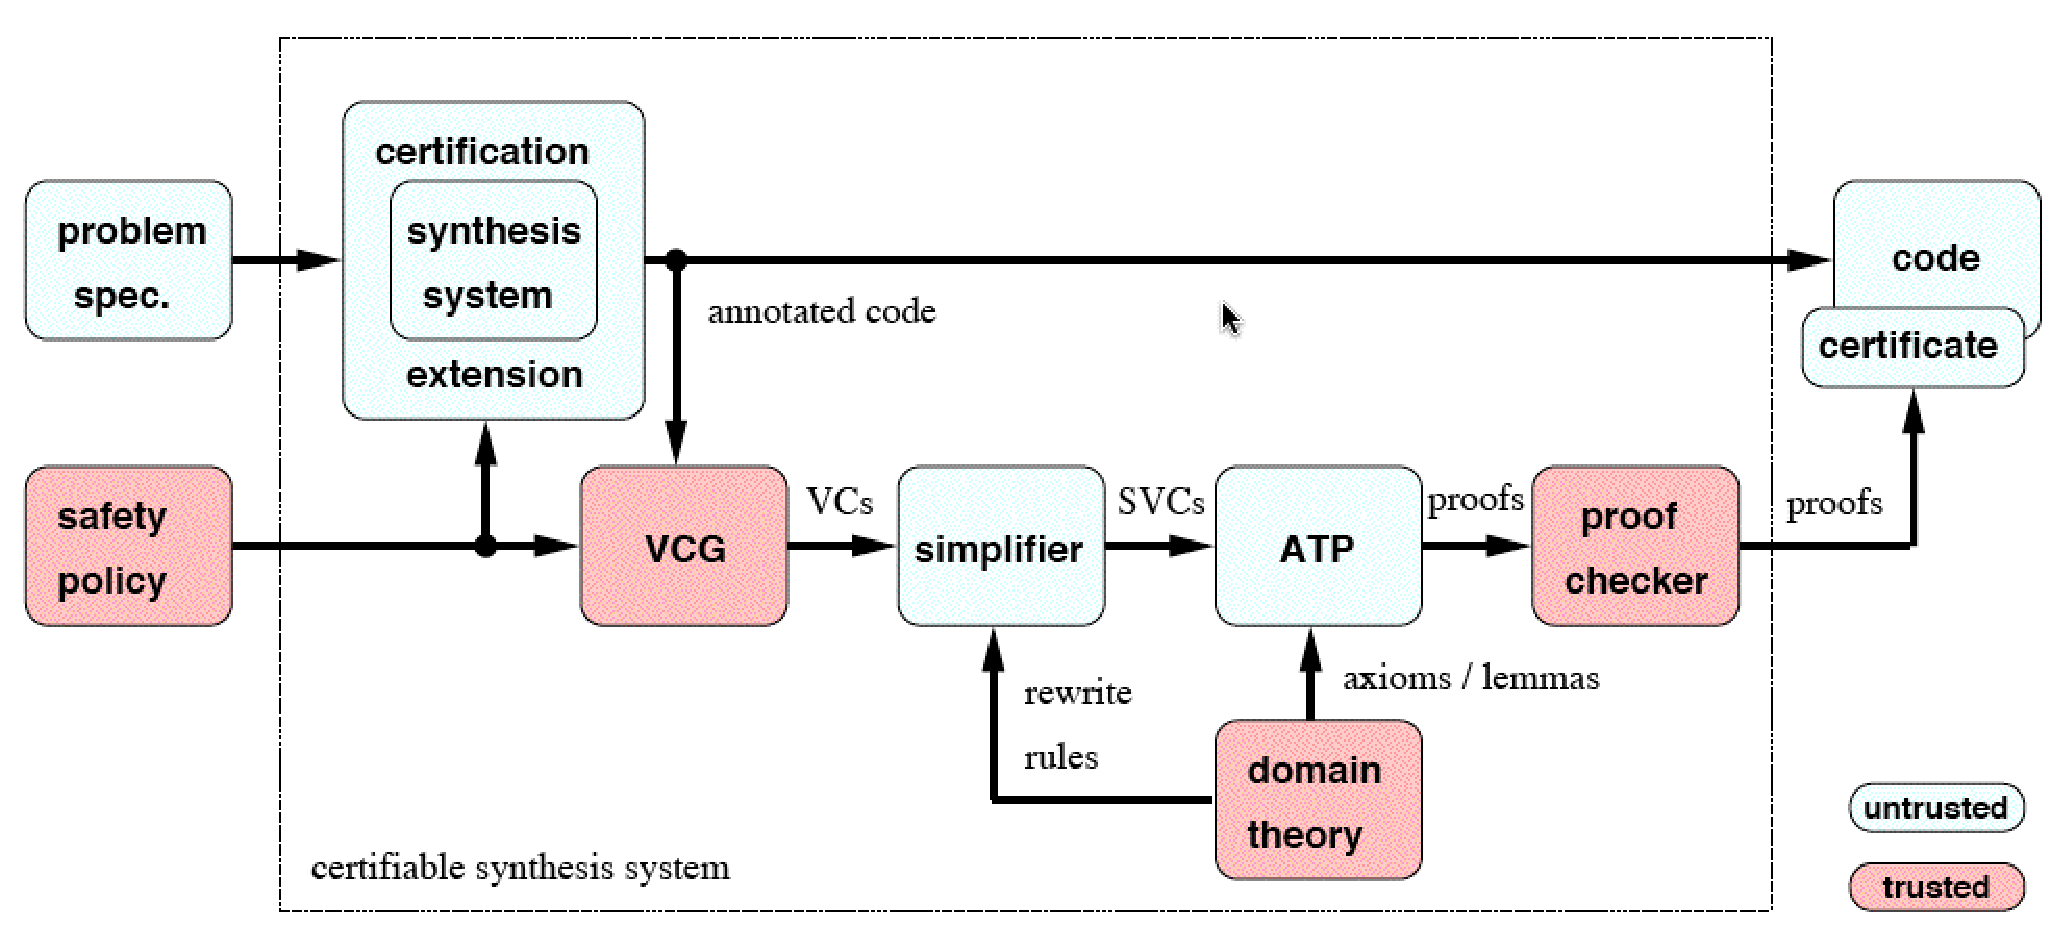
\includegraphics[width=0.6\textwidth]{NASACodeCertification}
% 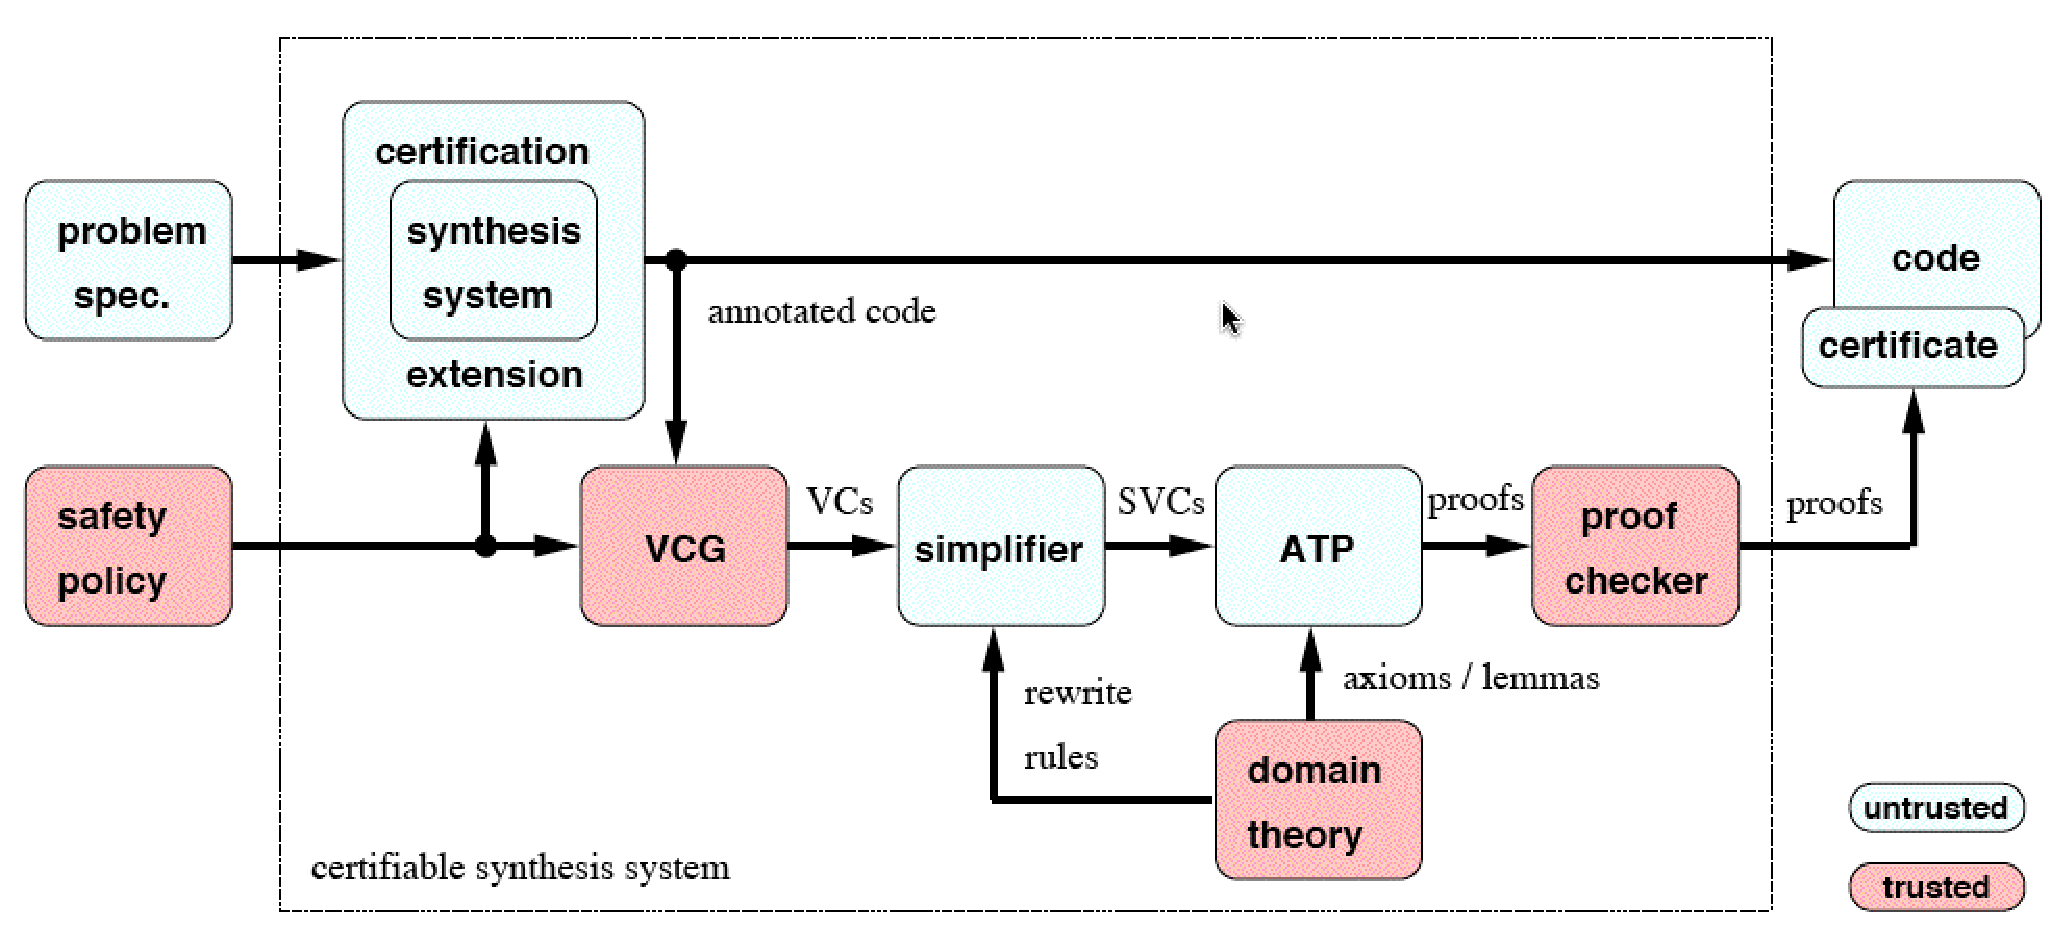
\includegraphics[width=0.8\columnwidth]{NASACodeCertification}   %FLAIRS
% \caption{Practical proof checking for program certification}
% \label{NASACodeCertification}
% \end{center}
% \end{figure}

At one top level, proofs can be divided into two types: Hilbert-style proofs that start at
axioms and derive theorems~\cite{End72}, and proofs-by-contradiction that negate the
conjecture to be proved and show that leads to a contradiction with the axioms~\cite{Men87}.
ATP systems that search for Hilbert-style proofs are often called ``natural deduction systems'',
e.g., THINKER~\cite{Pel98} and Muscadet~\cite{Pas01-IJCAR}.
Most contemporary high-performance ATP systems that search for a proof-by-contradiction, called
a refutation in this context, use a saturation based approach~\cite{Sch06}, e.g., E~\cite{SCV19} 
and Vampire~\cite{KV13}.
A complementary approach is taken in systems that build tableaux and closed connection 
matrices~\cite{FB+98}, e.g., leanCoP~\cite{Ott23} and Connect++~\cite{Hol23}.
The TPTP World (see Section~\ref{TPTP}) has an established format for writing Hilbert-style proofs 
and refutations~\cite{SS+06}, and has a tool for verifying proofs in that format (see
Section~\ref{Derivations}), but has not yet settled on a format for tableaux and connection
proofs.
One early proposal for a TPTP style format never gained traction~\cite{OS10}.
A more recent proposal~\cite{OH23} in the TPTP style provided some inspiration for the new format.

This paper is structured as follows:
Section~\ref{TPTP} introduces the TPTP World, providing the necessary background to the TPTP
language, explains the TPTP format for recording (non-tableau) derivations, and describes the
GDV and IDV tools for verifying and viewing derivations.
Section~\ref{Tableau} describes the new TPTP format for recording tableau proofs, and explains how
the format meets the requirements for easy reconstruction of the tableau, and for semantic 
verification of the tableau inference steps.
Section~\ref{SystemsTools} describes an ATP system that can output tableau proofs in the new
format, and explains how the GDV and IDV tools can be directly extended to verify and view
tableau proofs.
Section~\ref{Conclusion} concludes.

%--------------------------------------------------------------------------------------------------
\section{The TPTP World}
\label{TPTP}

The TPTP World~\cite{Sut24} is a well-established infrastructure that supports research, 
development, and deployment of Automated Theorem Proving (ATP) systems %(see 
%Section~\ref{TPTPWorld} for more details).
The TPTP World infrastructure includes
the TPTP language~\cite{SS+06},
the TPTP problem library~\cite{Sut09},
the TSTP solution library~\cite{Sut10},
the SZS ontologies~\cite{Sut08-KEAPPA},
the Specialist Problem Classes (SPCs) and problem difficulty ratings~\cite{SS01},
SystemOnTPTP~\cite{Sut00-CADE-17} and StarExec~\cite{SST14},
and the CADE ATP System Competition (CASC)~\cite{Sut16}.
The problem library is a large collection of Thousands of Problems for Theorem Proving -- hence 
the name. 
The problem library contains over 25000 problems from over 50 different domains, written in the 
TPTP language.
The problems are categorized into Specialist Problem Classes according to their syntactic and
logical status~\cite{Sut08-KEAPPA}.
The TSTP solution library is the result of running numerous ATP systems on that library and 
collecting their output. 
The solutions are categorized according to their logical and output form~\cite{Sut08-KEAPPA}.
The TPTP and TSTP libraries, with their categorizations, provide the basis for assigning a difficulty 
rating to each problem, according to the number of ATP systems that are able to solve 
it~\cite{SS01}.

The most salient feature of the TPTP World for this work is the TPTP language.
The TPTP language~\cite{Sut23-IGPL} is one of the keys to the success of the TPTP World.
The TPTP language is used for writing both problems and solutions,
which enables convenient communication between ATP systems and tools.
Originally the TPTP World supported only first-order clause normal form (CNF)
\cite{SS98-JAR}.
Over the years full first-order form (FOF)
\cite{Sut09}, 
typed first-order form (TFF)
\cite{SS+12,BP13-TFF1}, 
typed extended first-order form (TXF)
\cite{SK18}, 
typed higher-order form (THF)
\cite{SB10,KSR16}, 
and non-classical forms (NTF)~\cite{SF+22} have been added.
A general principle of the TPTP language is: ``We provide the syntax, you provide the semantics''.
As such, there is no a priori commitment to any semantics for each of the language forms, 
although in almost all cases the intended logic and semantics are well known.

Problems and solutions are built from {\em annotated formulae} of the form
\begin{center}
{\em language}{\tt (}{\em name}{\tt ,}
{\em role}{\tt ,}
{\em formula}{\tt ,}
{\em source}{\tt ,}
{\em useful\_info}{\tt )}
\end{center}
The {\em language}s supported are {\smalltt{cnf}} (clause normal form), {\smalltt{fof}}
(first-order form), {\smalltt{tff}} (typed first-order form), and {\smalltt{thf}}
(typed higher-order form).
The {\em role}, e.g., {\smalltt{axiom}}, {\smalltt{lemma}}, {\smalltt{conjecture}}, defines the 
use of the formula.
In a {\em formula}, terms and atoms follow Prolog conventions -- functions and predicates start 
with a lowercase letter or are {\tt '}single quoted{\tt '}, and variables start with an uppercase 
letter.
The language also supports interpreted symbols that either start with a {\tt \$}, e.g., the 
truth constants {\smalltt{\$true}} and {\smalltt{\$false}}, or are composed of 
non-alphabetic characters, e.g., integer/rational/real numbers such as 27, 43/92, -99.66.
The logical connectives in the TPTP language are
{\tt !>}, {\tt ?*}, {\tt @+}, {\tt @-}, {\tt !}, {\tt ?}, {\tt {\mytilde}}, {\tt |}, {\tt \&}, 
{\tt =>}, {\tt <=}, {\tt <=>}, and {\tt <{\mytilde}>}, for the mathematical connectives
$\Pi$, $\Sigma$, choice (indefinite description), definite description,
$\forall$, $\exists$, $\neg$, $\vee$, $\wedge$, $\Rightarrow$, $\Leftarrow$, $\Leftrightarrow$, 
and $\oplus$ respectively.
Equality and inequality are expressed as the infix operators {\tt =} and {\tt !=}.
The {\em source} and {\em useful\_info} are optional.
Figure~\ref{ExampleProblem} shows an example problem.

\begin{figure}[htb]
\centering
{\footnotesize
{\setlength{\baselineskip}{4mm}
\begin{verbatim}
%------------------------------------------------------------------------
fof(a1,axiom,         ~ ( ~q(b) & ? [X] : s(X) ) ).
fof(a2,axiom,         ( r & q(b) ) => ! [X] : ~p(X) ).
fof(a3,axiom,         p(c) | ! [Y] : ( ~q(c) & q(Y) ) ).
fof(a4,axiom,         ~q(c) => ~q(b) ).
fof(a5,axiom,         p(c) => r ).
fof(prove,conjecture, ! [X] : ( ~s(X) & ~q(b) & p(c) ) ).
%------------------------------------------------------------------------
\end{verbatim}
}}
\caption{An example problem in TPTP format}
\label{ExampleProblem}
\end{figure}

%--------------------------------------------------------------------------------------------------
\subsection{The TPTP Format for Derivations}
\label{Derivations}

A derivation written in the TPTP language is a list of annotated formulae. 
The leaves of a derivation DAG are typically have a role {\smalltt axiom} or {\smalltt conjecture}, 
and the role for inferred formulae is typically one of {\smalltt negated\_conjecture} (also used 
for leaves in CNF) or {\smalltt plain} for inferred formulae. 
The source is either a {\smalltt file} record for leaves or an {\smalltt inference} record for 
inferred formulae.
A {\smalltt file} record contains the problem file name and the corresponding annotated formulae 
name in the problem file.
An {\smalltt inference} record contains the inference rule name, a list of useful inference 
information, and a list of the inference parents.
The inference parents can be annotated formulae names, and nested {\smalltt inference} records.
Common types of useful inference information are the semantic relationship of the inferred formula 
to its parents as an SZS ontology value~\cite{Sut08-KEAPPA} in a {\smalltt status} record, 
special information about recognized types of complex inference rules, e.g., Skolemization and
explicit splitting, and details of new symbols introduced in the inference.
The use of SZS values is core to GDV's approach to verification, described below.

Figure~\ref{ExampleClausification} shows the transformation to CNF of the problem in 
Figure~\ref{ExampleProblem}, which is used in the refutation discussed here, and the tableau
proof in Section~\ref{Tableau}.
Points of note:
all the leaf formulae except {\tt a4} and {\tt a5} are copies of formulas in the problem;
{\tt a4} and {\tt a5} are easily derived from the corresponding problen formulae;
many of the formulae are inferred with SZS status {\smalltt{thm}}, i.e., they are logical 
consequences of their parents;
the negated conjecture {\smalltt c\_0\_7} is inferred with SZS status {\smalltt{cth}} --
its negation is a logical consequence of its parent;
the Skolemized formula {\smalltt c\_0\_11} is inferred with SZS status {\smalltt{esa}} --
it is equisatisfiable with its parent;

\begin{figure}[htb]
\centering
{\footnotesize
{\setlength{\baselineskip}{4mm}
\begin{verbatim}
%------------------------------------------------------------------------
fof(a1,axiom,              ~ ( ~q(b) & ? [X] : s(X) ),
    file('PaperFOF.p',a1) ).
fof(a2,axiom,              ( r & q(b) ) => ! [X] : ~p(X),
    file('PaperFOF.p',a2) ).
fof(a3,axiom,              p(c) | ! [Y] : ( ~q(c) & q(Y) ),
    file('PaperFOF.p',a3) ).
fof(a4,axiom,              ~q(c) => ~q(b),
    file('PaperFOF.p',a4) ).
fof(a5,axiom,              p(c) => r,
    file('PaperFOF.p',a5) ).
fof(prove,conjecture,      ! [X] : ( ~s(X) & ~q(b) & p(c) ),
    file('PaperFOF.p',prove) ).

fof(nc1,negated_conjecture, ~ ! [X] : ( ~s(X) & ~q(b) & p(c) ),
    inference(negate,[status(cth)],[prove]) ).
fof(nc2,negated_conjecture, ? [X] : ~ ( ~s(X) & ~q(b) & p(c) ),
    inference(negate,[status(thm)],[nc1]) ).
fof(nc3,negated_conjecture, ~ ( ~s(sK1) & ~q(b) & p(c) ),
    inference(skolemize,[status(esq),new_symbols(skolem,[sK1]),
skolemized(X)],[nc2]) ).

cnf(c1,plain,               ( q(b) | ~s(X) ),
    inference(clausify,[status(thm)],[a1]) ).
cnf(c2,plain,               ( ~q(b) | ~p(X) | ~r ),
    inference(clausify,[status(thm)],[a2]) ).
cnf(c3,plain,               ( p(c) | ~q(c) ),
    inference(clausify,[status(thm)],[a3]) ).
cnf(c4,plain,               ( p(c) | q(Y) ),
    inference(clausify,[status(thm)],[a3]) ).
cnf(c5,plain,               ( q(c) | ~q(b) ),
    inference(clausify,[status(thm)],[a4]) ).
cnf(c6,plain,               ( r | ~p(c) ),
    inference(clausify,[status(thm)],[a5]) ).
cnf(c7,negated_conjecture,  ( s(sK1) | q(b) | ~p(c) ),
    inference(clausify,[status(thm)],[nc3]) ).
%------------------------------------------------------------------------
\end{verbatim}
}}
\caption{Clausification for CNF-based proofs of the problem in Figure~\ref{ExampleProblem}}
\label{ExampleClausification}
\end{figure}

Figure~\ref{ExampleDerivation} shows the final steps of the refutation found by E~3.2.5 for the
problem in Figure~\ref{ExampleProblem}, following the transformation to CNF shown in 
Figure~\ref{ExampleClausification}.\footnote{%
The full refutation can be generated in \href{https://tptp.org/cgi-bin/SystemOnTPTP}{SystemOnTPTP}}
Points of note:
many of the formulae are inferred with SZS status {\smalltt{thm}}, i.e., they are logical 
consequences of their parents;
several of the inferred formulae, e.g., {\smalltt{c\_0\_23}}, have nested {\smalltt{inference}}
records -- the intermediate inferred formulae have not been output. 

\begin{figure}[htb]
\centering
{\footnotesize
{\setlength{\baselineskip}{4mm}
\begin{verbatim}
%------------------------------------------------------------------------
cnf(c_0_23,plain,              ~r | ~q(b),
    inference(csr,[status(thm)],
[inference(spm,[status(thm)],[c_0_18, c_0_19]), c_0_20])).

cnf(c_0_24,negated_conjecture, q(b) | ~q(c),
    inference(spm,[status(thm)],[c_0_21, c_0_19])).

cnf(c_0_25,plain,              r | ~p(c),
    inference(split_conjunct,[status(thm)],[c_0_22])).

cnf(c_0_26,negated_conjecture, ~r | ~q(c),
    inference(spm,[status(thm)],[c_0_23, c_0_24])).

cnf(c_0_27,plain,              q(X1) | p(c),
    inference(split_conjunct,[status(thm)],[c_0_14])).

cnf(c_0_28,plain,              ~q(c),
    inference(csr,[status(thm)],
[inference(spm,[status(thm)],[c_0_25, c_0_19]), c_0_26])).

cnf(c_0_29,plain,              r | q(X1),
    inference(spm,[status(thm)],[c_0_25,c_0_27]) ).

cnf(c_0_30,plain,              r,
    inference(spm,[status(thm)],[c_0_28,c_0_29]) ).

cnf(c_0_31,plain,              ~q(b),
    inference(cn,[status(thm)],
[inference(rw,[status(thm)],[c_0_23,c_0_30])]) ).

cnf(c_0_32,negated_conjecture, q(X1),
    inference(sr,[status(thm)],
[inference(spm,[status(thm)],[c_0_21,c_0_27]),c_0_31]) ).

cnf(c_0_33,plain,              $false,
    inference(cn,[status(thm)],
[inference(rw,[status(thm)],[c_0_31,c_0_32])]),
    [proof] ).
%------------------------------------------------------------------------
\end{verbatim}
}}
\caption{The final steps E 3.2.5's refutation of Figure~\ref{ExampleProblem}}
\label{ExampleDerivation}
\end{figure}

The GDV derivation verifier~\cite{Sut06} verifies proofs by refutation.
% Most recently it has been developed to produce LambdaPi terms that can be independently verified 
% using the {\smalltt lambdapi} checker.~\cite{SBB25}
GDV's input is a TPTP format refutation, and optionally (required for complete verification) the 
problem for which the proof was produced.
GDV checks a TPTP proof in four verification phases: structural verification, leaf verification,
rule-specific verification, and inference verification.
Many of the checks rely on a ``check-by-ATP'', which calls a trusted ATP system -- either a theorem 
prover or a model finder.
The default trusted theorem provers and model finders used by GDV are Otter~\cite{McC03-Otter}
and E~\cite{SCV19} for theorem proving, Paradox~\cite{CS18}, Vampire~\cite{KV13}, and
Nitpick~\cite{BN10-ITP} for model finding.
These systems have become trusted through the process described in \cite{SBB25}.
Structural verification deals with non-logical aspects of a proof, checking whether the
the annotated formulae of the proof have the right format and relationships, e.g., all the 
parents of inferred formulae exist, the refutation is acyclic. 
Leaf verification deals with the leaves of the derivation, and their relationship with
the problem annotated formulae, e.g., check-by-ATP that the leaf axioms are satisfiable, and 
that leaves are copies of problem formulae or can be proved from problem formulae using a 
check-by-ATP.
Rule specific verification deals with inference rules that require special treatment, e.g.,
explicit splitting~\cite{Wei01} and Skolemization. 
Inference verification deals with the various types of inferences that are made by ATP
systems in a proof.
Examples of checks are: for inference steps with SZS status {\smalltt{thm}} check-by-ATP that the 
inferred formula can be proved from the parent formulae, for inference steps with SZS status 
{\smalltt{cth}} check-by-ATP that the negation of the inferred formula can be proved from the 
parent formulae.

% \begin{figure*}[htb]   %FLAIRS
% \begin{center}
% 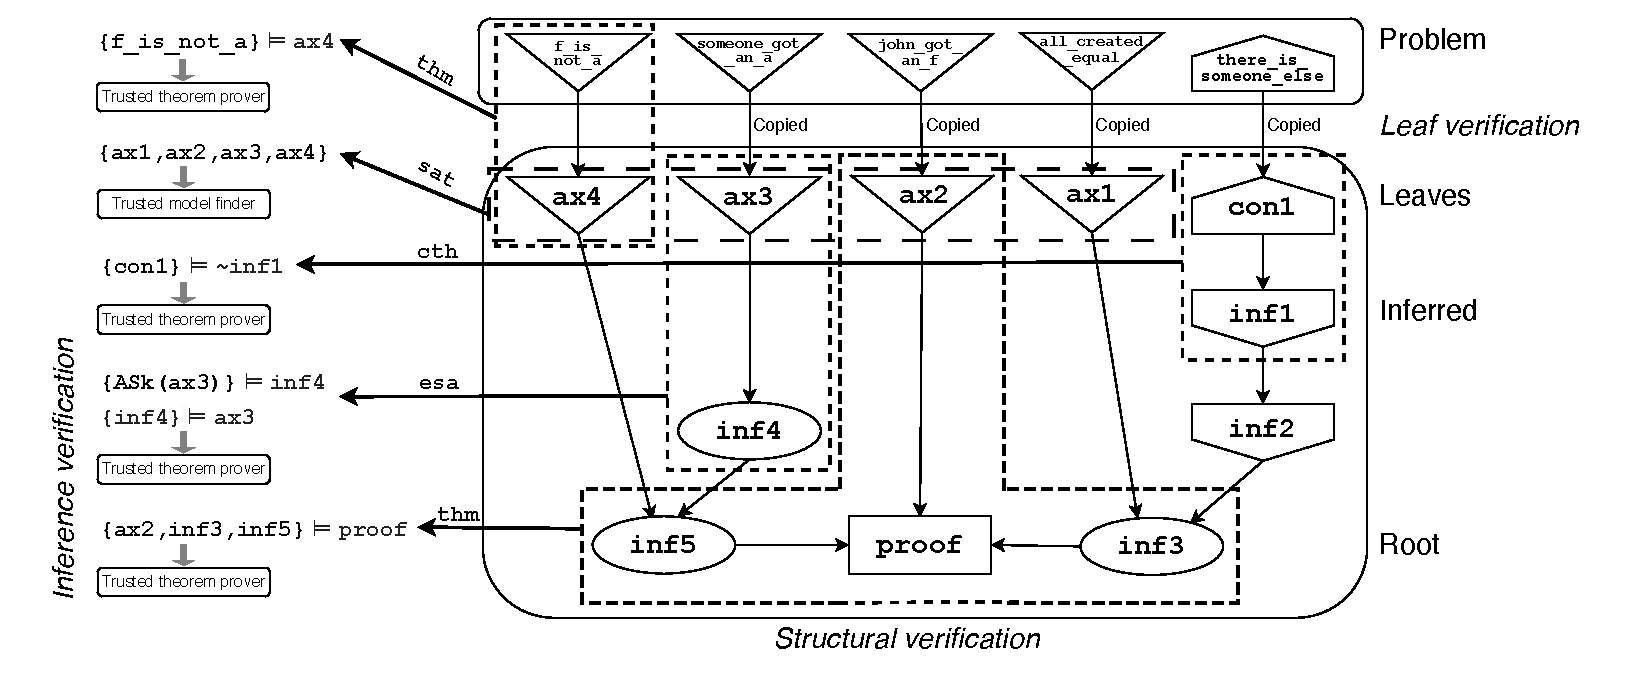
\includegraphics[width=1.0\textwidth]{GDVArchitecture}
% \caption{GDV architecture}
% \label{GDVArchitecture}
% \end{center}
% %EASYCHAIR \end{figure}
% \end{figure*}   %FLAIRS

The IDV Interactive Derivation Viewer~\cite{TPS07} provides a graphical rendering of a proof
DAG, with features that allow the user to examine the proof structure in various way, 
including identification of ``interesting'' steps in the proof~\cite{PGS06}.
Figure~\ref{Refutation} shows the IDV rendering of the (full version of the) refutation in 
Figure~\ref{ExampleDerivation}

\begin{figure}[htb]
\centering
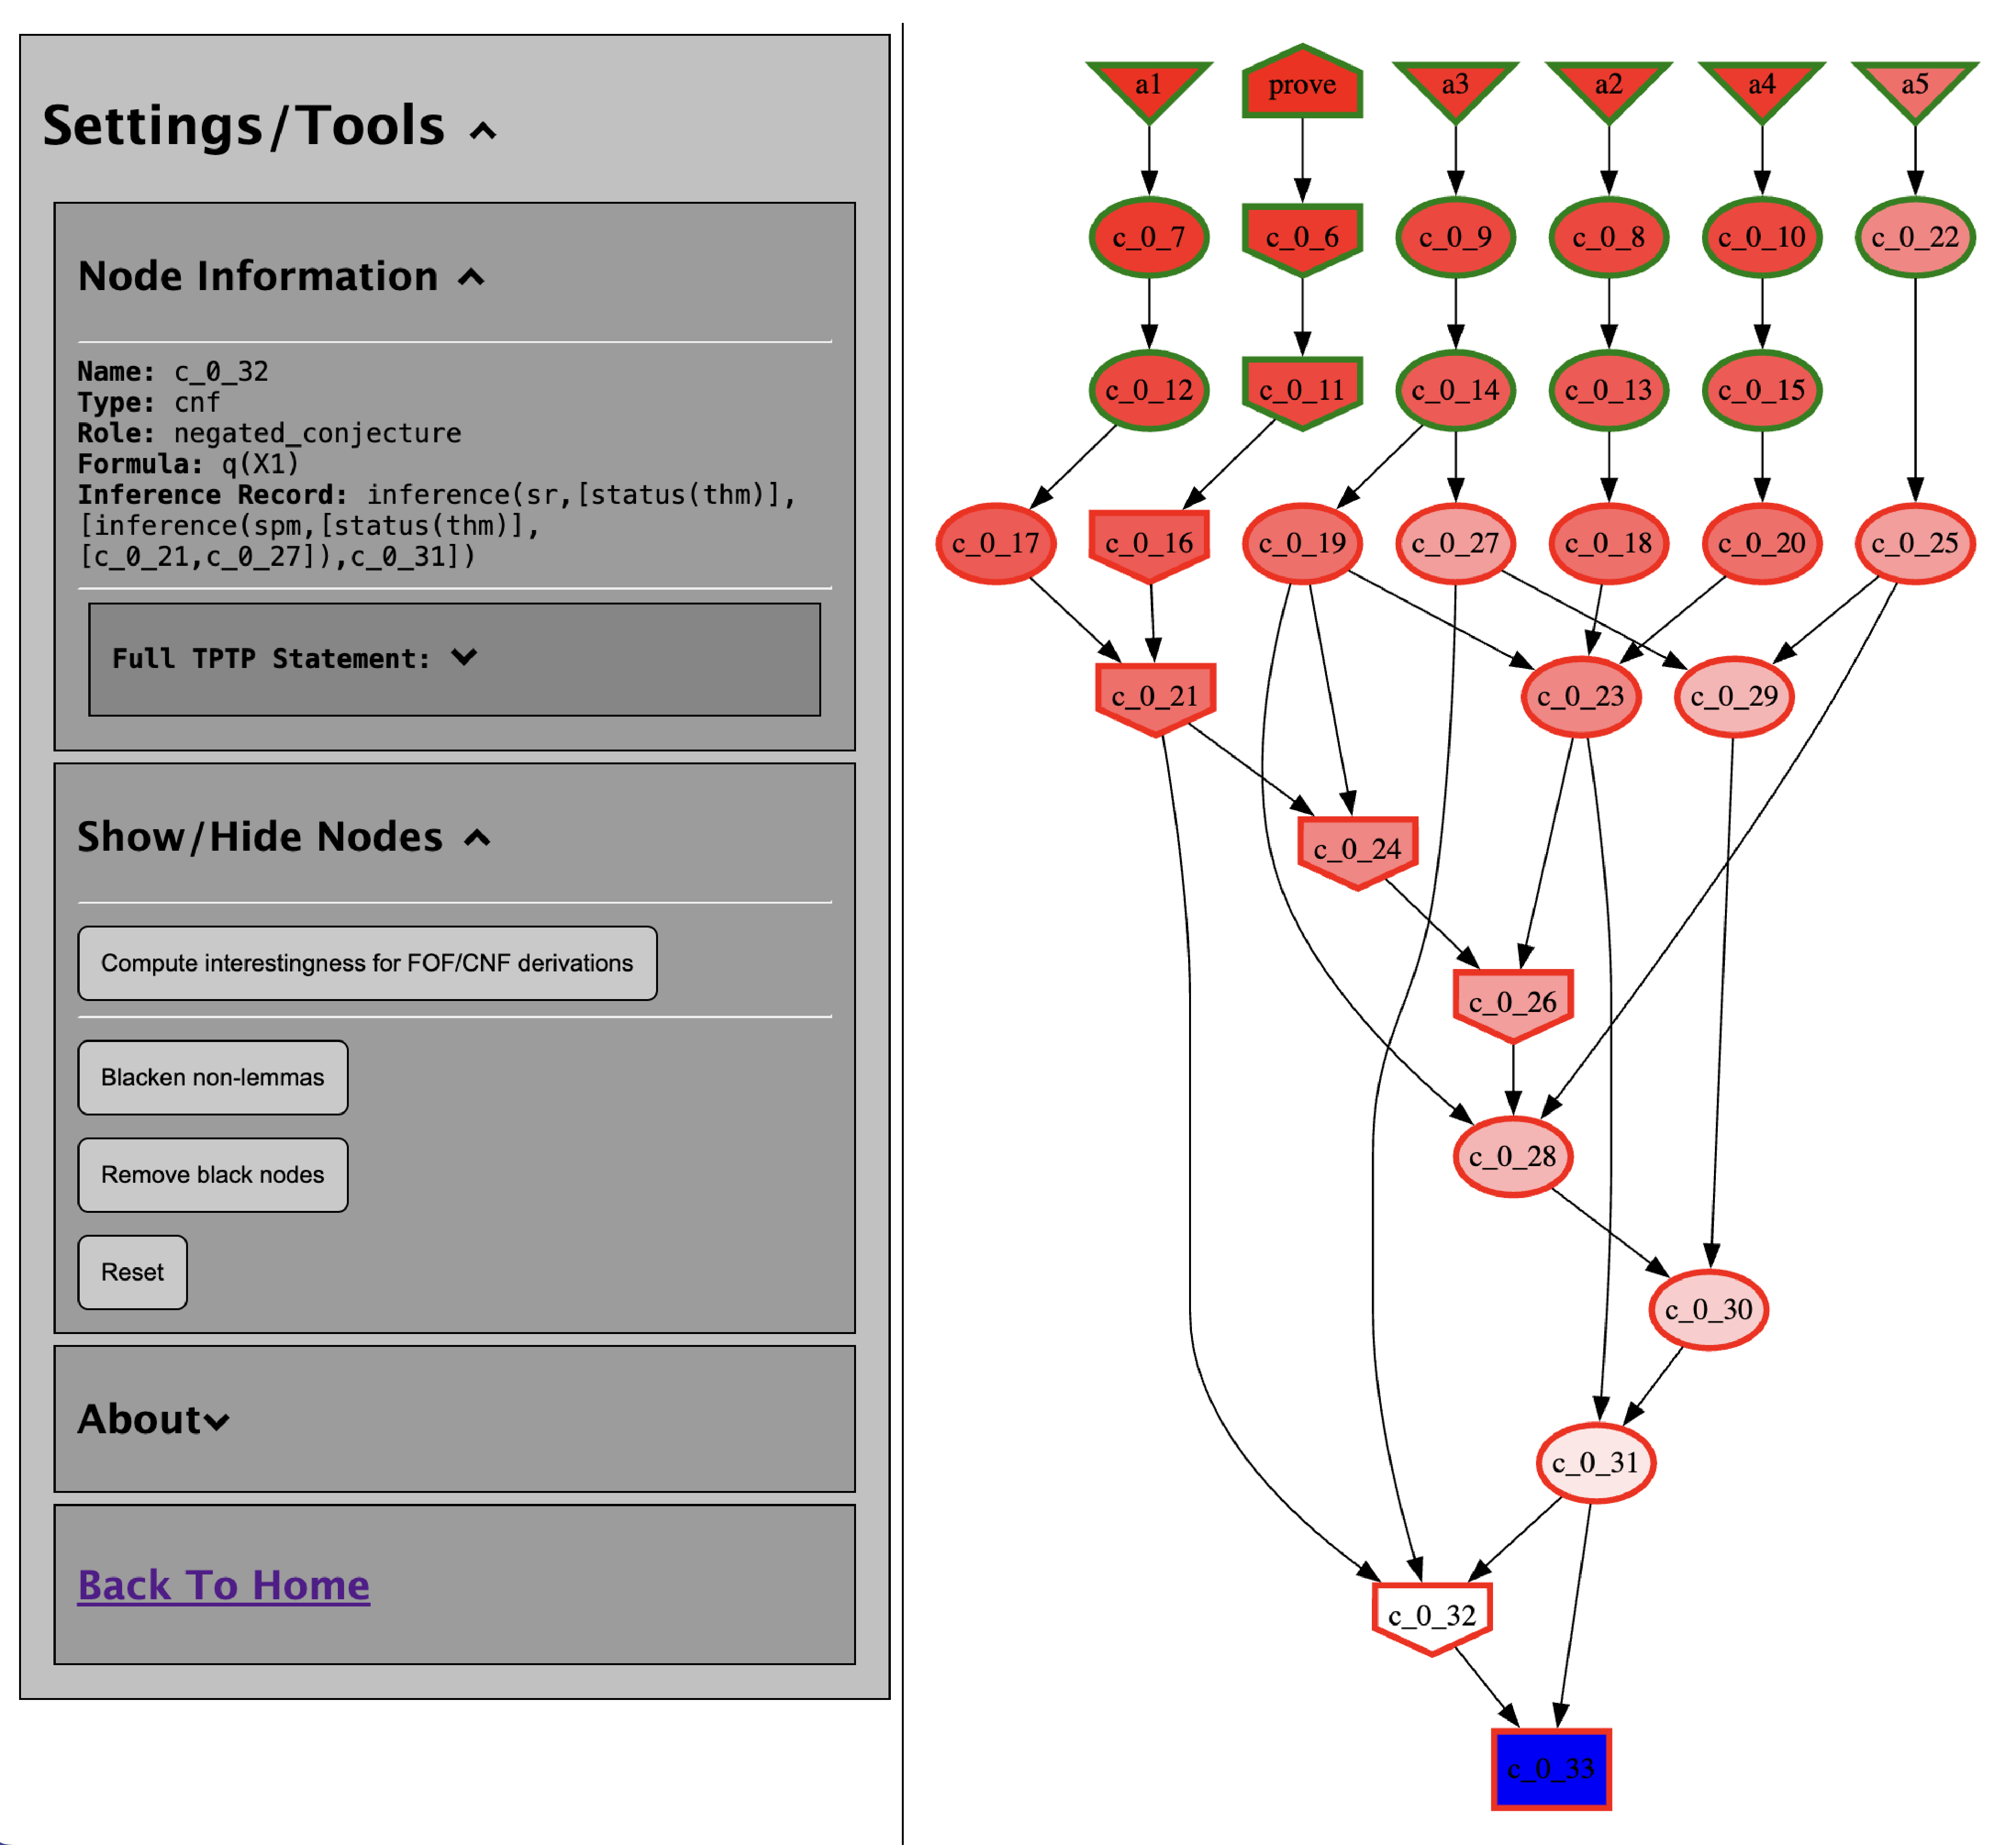
\includegraphics[width=0.8\textwidth]{PaperFOFIDV.pdf}
\vspace*{-1em}
\caption{IDV rendering of the (full version of the) refutation in Figure~\ref{ExampleDerivation}}
\label{Refutation}
\end{figure}

%--------------------------------------------------------------------------------------------------
\section{The (new) TPTP Format for Tableau Proofs}
\label{Tableau}

There were three primary requirements for the new format for tableau proofs:
\begin{enumerate}
\item Easy reconstruction of the tableau.
\item Sufficient information for structural verification of the closed tableau.
\item Sufficient information for semantic verification of the inference steps.
\end{enumerate}
Additional requirements adopted from~\cite{OH23} are:
\begin{enumerate}[resume]
\item Concise and simple enough for a natural representation of proofs.
\item Readable by humans as well as ATP tools.
\end{enumerate}
One early proposal for a TPTP style format~\cite{OS10} met requirement~1, but fell short
of requirements~2 and~3 due to the omission of some necessary details. 
As claimed in~\cite{OH23}, that early proposal might have also failed to meet requirements~4 and~5.
Another existing TPTP style format is the leanTPTP format output by the leanCoP ATP 
system~\cite{OB03}.
The leanTPTP format definitely meets requirement~4, but omits the information required for 
requirements~1,~2, and~3.
A more recent proposal~\cite{OH23} in the TPTP style provided some inspiration for the new format,
but left some important information as implicit, which is made explicit in the new format.
The new format aims to meet all the requirements.

Figure~\ref{TableauPicture} shows the tableau for the problem in Figure~\ref{ExampleProblem}.
Figure~\ref{ExampleTableau} shows the TPTP format for the tableau, following the transformation
to CNF shown in Figure~\ref{ExampleClausification}.
The labels in square brackets in Figure~\ref{TableauPicture} identify the literals in the 
annotated formulae in Figure~\ref{ExampleTableau}.
The solid rightward arrows point to the lemmas that are created. 
Note that lemmas can be used only below the parent node of where they are created. 
In Figure~\ref{ExampleTableau} the cases where the lemmas are used are shown with dashed arrows.
The tableau in Figure~\ref{TableauPicture} has the variables instantiated as they would be when 
the tableau is closed.

\begin{figure}[htb]
\centering
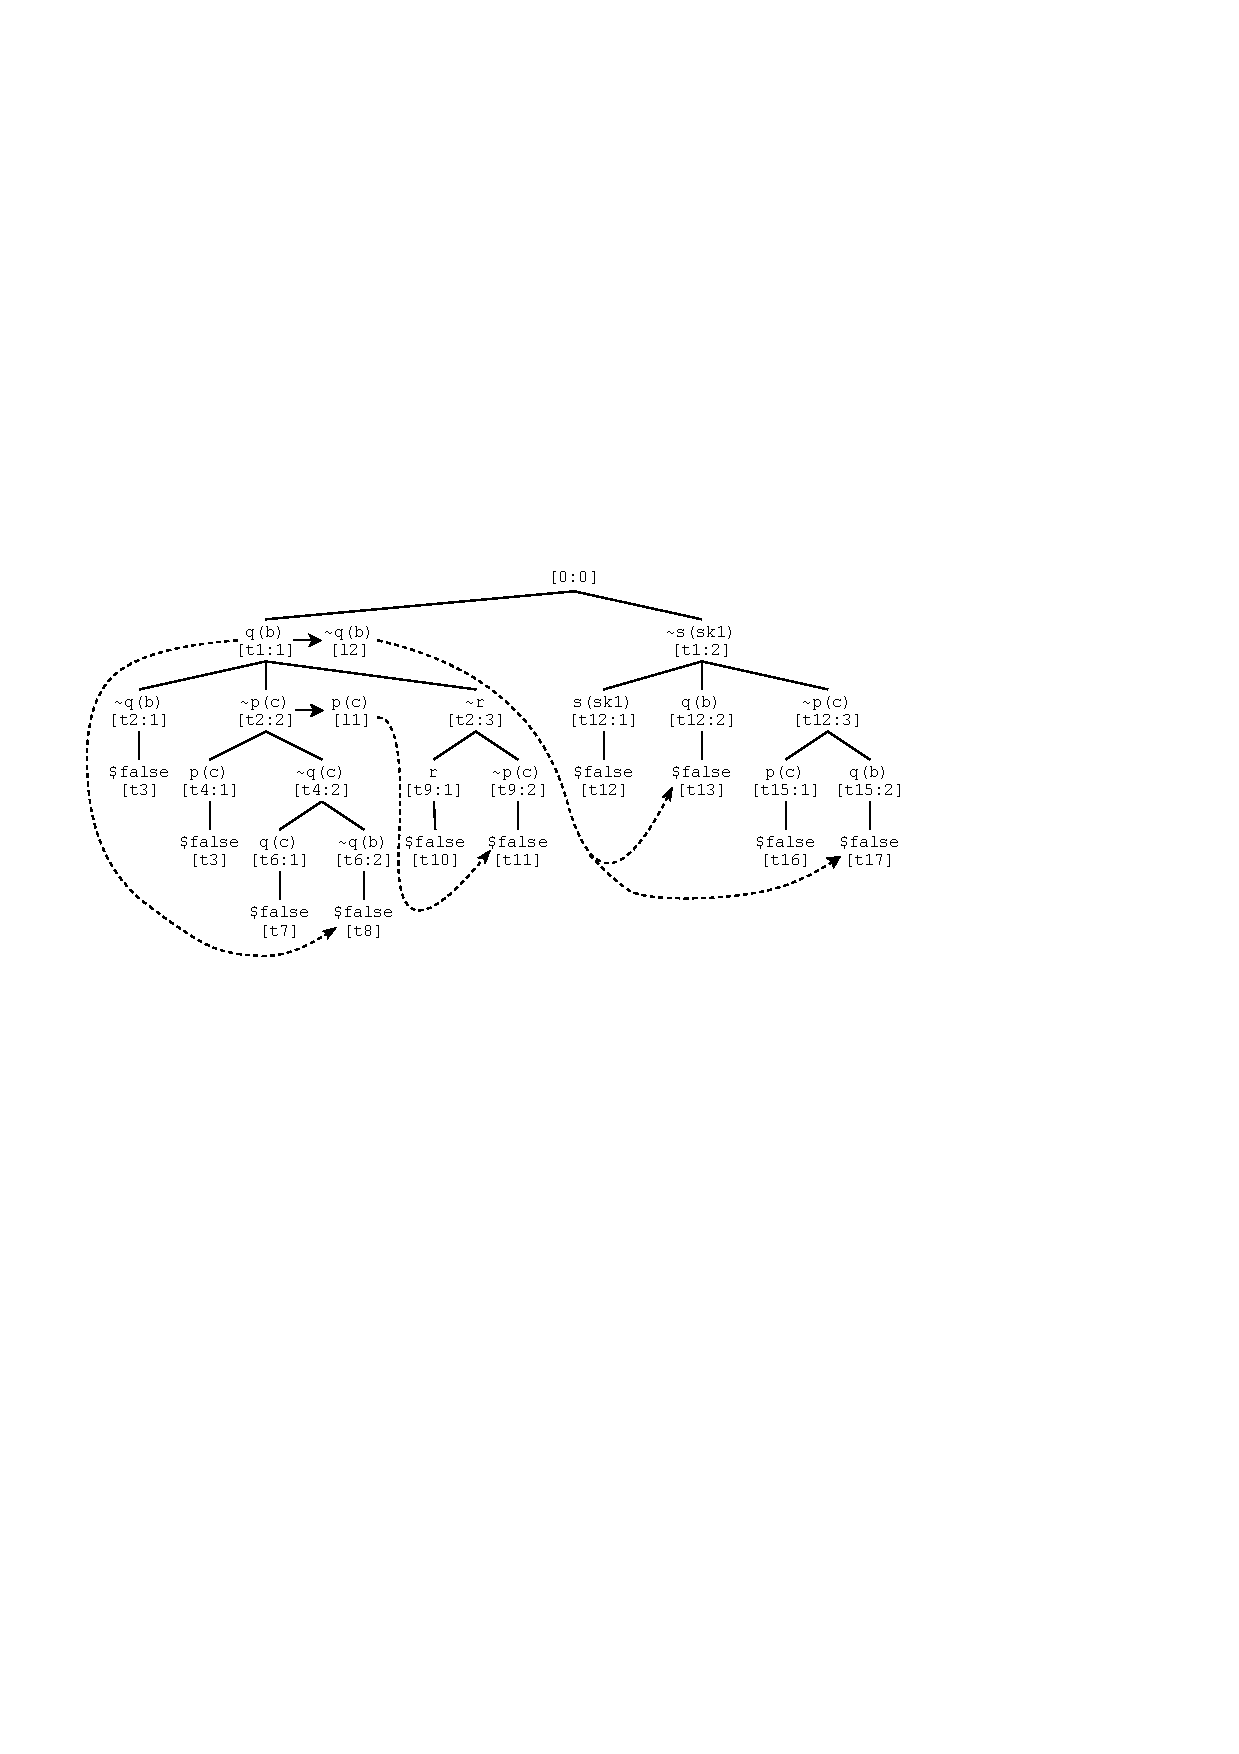
\includegraphics[width=1.0\textwidth]{Tableu_updated.pdf}
\vspace*{-1em}
\caption{Tableau for the problem in Figure~\ref{ExampleProblem}}
\label{TableauPicture}
\end{figure}

The TPTP format recognizes six inference rules, which are described below.
The inference record of each annotated formula records the name of the rule used, the SZS status 
of the inferred formula wrt it parents, the path from the root to the node above, and the 
inference parents.  
The SZS status and parent information makes it possible to use semantic verification of each 
inference, and the path information makes it easy to reconstruct the tableau.
The point at which a variable becomes instantiated can optionally be recorded with a {\tt bind()} 
record, e.g., 
{\footnotesize
\begin{verbatim}
cnf(t4,plain,              p(c) | ~ q(c),
    inference(extension,[status(thm),path([t2:2,t1:1]),bind(X,c)],[c3]) ).
\end{verbatim}
}
\noindent
notes that the variable {\smalltt{X}} in {\smalltt{t2} is bound to {\smalltt{c}} (assuming 
variables have been renamed apart so that it is clear that the {\smalltt X} is in {\smalltt{t2}}).
% AAAARGH, WE NEED TO GET THIS VERY CLEAR.

\paragraph{{\tt start}:} The initial clause below the root node.
For example, in Figure~\ref{ExampleTableau} {\smalltt{t1}} starts the tableau.
The path to this point is recorded as {\smalltt{path([0:0])}}, indicating that the node above
is the root node.
The logical parent is recorded as {\smalltt{[c1]}}. 
The inference has status {\smalltt{thm}}, i.e., {\smalltt{t1}} is a logical consequence of its
parent.
{\tt start} can be viewed as a special form of {\tt extension}, described next.

\paragraph{{\tt extension}:} The standard tableau extension rule.
For example, in Figure~\ref{ExampleTableau} {\smalltt{t2}} extends from the first literal 
{\smalltt{q(b)}} of {\smalltt{t1}} to the 1st literal {\smalltt{{\mytilde}q(b)}} of {\smalltt{c2}}.
The path to this point is recorded as {\smalltt{path([t1:1])}}. 
The logical parent is recorded as {\smalltt{[c2]}}. 
The inference has status {\smalltt{thm}}, i.e., {\smalltt{t2}} is a logical consequence of its
parent.

\paragraph{{\tt connection}:} Explicitly close the branch of the contradiction of an extension.
For example, Figure~\ref{ExampleTableau} {\smalltt{t3}} closes the branch of the contradiction 
between {\smalltt{q(b)}} and {\smalltt{{\mytilde}q(b)}} in the extension {\smalltt{t2}}.
The path to this point is recorded as {\smalltt{path([t2:1,t1:1])}}.
The logical parents are recorded as {\smalltt{[t2:1,t1:1]}}, meaning the 1st literal of 
{\smalltt{t2}} and the 1st literal of {\smalltt{t1}}. 
The inference has status {\smalltt{thm}}, i.e., {\smalltt{t3}} is a logical consequence of its
parents. 
{\tt connection} can be viewed as a degenerate form of {\tt reduction}, described next.

\paragraph{{\tt reduction}:} The standard tableau reduction rule.
For example, Figure~\ref{ExampleTableau} {\smalltt{t8}} closes the branch of the contradiction 
between the 2nd literal {\smalltt{{\mytilde}q(b)}} of {\smalltt{t6}} and the 1st literal 
{\smalltt{q(b)}} of {\smalltt{t1}}.
The path to this point is recorded as {\smalltt{path([t6:2,t4:2,t2:2,t1:1])}}.
The logical parents are recorded as {\smalltt{[t6:2,t1:1]}}, meaning the 2nd literal of 
{\smalltt{t6}} and the 1st literal of {\smalltt{t1}}. 
The inference has status {\smalltt{thm}}, i.e., {\smalltt{t8}} is a logical consequence of its 
parents.

\paragraph{{\tt lemma}:} The creation of a unit lemma when a branch is closed.
For example, Figure~\ref{ExampleTableau} {\smalltt{l1}} is the lemma {\smalltt{p(c)}} created 
when the branch rooted at {\smalltt{t2:2}} is closed.
The lemma is the negation of the 2nd literal {\smalltt{{\mytilde}p(c)}} of {\smalltt{t2}}.
The path to this point is recorded as {\smalltt{path([t2:2,t1:1])}}.
As the node {\smalltt{t1:1}} is used in a reduction in closing the branch, the lemma is
available only below {\smalltt{t1:1}}, recorded as {\smalltt{below(t1:1)}}.
The logical parent is recorded as {\smalltt{[t4:1]}}, meaning the 1st literal of
{\smalltt{t4}} that is the negation of the 2nd literal {\smalltt{{\mytilde}p(c)}} of {\smalltt{t2}}.
The inference has status {\smalltt{thm}}, i.e., {\smalltt{l1}} is a logical consequence of its 
parents.

\paragraph{{\tt lemma\_extension}:} Use of a lemma to close a branch.
For example, Figure~\ref{ExampleTableau} {\smalltt{t11}} is the result of using the lemma 
{\smalltt{l1}} to close the branch down to {\smalltt{9:2}}.
The lemma {\smalltt{l1}} can be used because {\smalltt{9:2}} is below {\smalltt{t1:1}}.
The path to this point is recorded as {\smalltt{path([l1:1,t9:2,t2:3,t1:1])}}.
The logical parents are recorded as {\smalltt{[l1:1,t9:2]}}, meaning the 1st literal 
{\smalltt{p(c)}} of {\smalltt{l1}} and the 2nd literal {\smalltt{{\mytilde}p(c)}} of 
{\smalltt{t9}}.
The inference has status {\smalltt{thm}}, i.e., {\smalltt{t11}} is a logical consequence of its
parents.
{\tt lemma\_extension} can be viewed as a special form of {\tt extension}.

\begin{figure}[h!]
\centering
{\scriptsize
{\setlength{\baselineskip}{3mm}
\begin{verbatim}
%--------------------------------------------------------------------------------------------
cnf(t1,plain,               q(b) | ~s(X),
    inference(start,[status(thm),path([0:0])],[c1]) ).

cnf(t2,plain,               ~q(b) | ~p(X) | ~r,
    inference(extension,[status(thm),path([t1:1,0:0])],[c2]) ).

cnf(t3,plain,               $false,
    inference(connection,[status(thm),path([t2:1,t1:1,0:0])],[t2:1,t1:1]) ).

cnf(t4,plain,               p(c) | ~q(c),
    inference(extension,[status(thm),path([t2:2,t1:1,0:0])],[c3]) ).

cnf(t5,plain,               $false,
    inference(connection,[status(thm),path([t4:1,t2:2,t1:1,0:0])],[t4:1,t2:2]) ).

cnf(t6,plain,               q(c) | ~q(b),
    inference(extension,[status(thm),path([t2:2,t1:1,0:0])],[c5]) ).

cnf(t7,plain,               $false,
    inference(connection,[status(thm),path([t6:1,t4:2,t2:2,t1:1,0:0])],[t6:1,t4:2]) ).

cnf(t8,plain,               $false,
    inference(reduction,[status(thm),path([t6:2,t4:2,t2:2,t1:1,0:0])],[t6:2,t1:1]) ).

cnf(l1,plain,               p(c),
    inference(lemma,[status(thm),path([t2:2,t1:1,0:0]),below(t1:1)],[t4:1]) ).

cnf(t9,plain,               r | ~p(c),
    inference(extension,[status(thm),path([t2:3,t1:1,0:0])],[c6]) ).

cnf(t10,plain,              $false,
    inference(connection,[status(thm),path([t9:1,t2:3,t1:1,0:0])],[t9:1,t2:3]) ).

cnf(t11,plain,              $false,
    inference(lemma_extension,[status(thm),path([l1:1,t9:2,t2:3,t1:1,0:0])],[l1:1,t9:2]) ).

cnf(l2,plain,               ~q(b),
    inference(lemma,[status(thm),path([t1:1,0:0]),below(0:0)],[t2:1]) ).

cnf(t12,plain,              s(sK1) | q(b) | ~p(c),
    inference(extension,[status(thm),path([t1:2,0:0])],[c7]) ).

cnf(t13,plain,              $false,
    inference(connection,[status(thm),path([t12:1,t1:2,0:0])],[t12:1,t1:2]) ).

cnf(t14,plain,              $false,
    inference(lemma_extension,[status(thm),path([l2:1,t12:2,t1:2,0:0])],[l2:1,t12:2]) ).

cnf(t15,plain,              p(c) | q(Y),
    inference(extension,[status(thm),path([t12:3,t1:2,0:0])],[c4]) ).

cnf(t16,plain,              $false,
    inference(connection,[status(thm),path([t15:1,t12:3,t1:2,0:0])],[t15:1,t2:3]) ).

cnf(t17,plain,              $false,
    inference(lemma_extension,[status(thm),path([l2:1,t15:2,t12:3,t1:2,0:0])],[l2:1,t15:2]) ).
%--------------------------------------------------------------------------------------------
\end{verbatim}
}}
\caption{Tableau in TPTP format, for the problem in Figure~\ref{ExampleProblem}}
\label{ExampleTableau}
\end{figure}

%--------------------------------------------------------------------------------------------------
\section{ATP Systems and Tools}
\label{SystemsTools}

% Sean:
Connect++ is a prover for first-order logic based on clausal connection calculus.~\cite{Hol23} 
The advantages of connection provers, with respect to their goal-oriented search and ability to 
produce readable proofs, are well-known
Connect++ supports restricted backtracking, restriction of start clauses, reordering, iterative 
deepening by path length or tree depth.
Connect++ supports the use of arbitrary search schedules, and can read these from a file in a 
simple format.
It deals with equality by detecting its use in the input file and adding the necessary axioms.
Most relevant to work, Connect accepts input in TPTP format, and {\em outputs closed tableau in
the new format}.
Connect++ is implemented in C++, and is open source under the GNU General Public License (GPL) 
Version 3.\footnote{%
\href{https://www.cl.cam.ac.uk/~sbh11/connect++.html}{\smalltt{www.cl.cam.ac.uk/~sbh11/connect++.html}}}.

The extension of GDV to verify tableau requires extending the structural verification phase,
and a minor change to inference verification.
Leaf verification remains unchanged, and the rule-specific steps of derivation verification
are naturally inapplicable.
Structural verification of a tableau requires checking:
\begin{packed_itemize}
\item All inference parents exist, in particular that the specified literals exist.
\item The {\smalltt{path}} records define an acyclic DAG, without contradictions in the paths.
\item All paths end at the root {\smalltt{0:0}} node.
\item The tableau is closed, i.e., every branch ends at a {\smalltt{\$false}} formula.
\item All {\tt lemma\_extension} steps use lemmas that are below the specified node in the tableau.
\end{packed_itemize}
Semantic verification is essentially the same as for derivations, with the small additional need 
to extract the specified literals from inference parents.

The extension of IDV to an Interactive Tableau Viewer (ITV) is quite simple, and will be 
completed as soon as my undergraduate developers have time.

%--------------------------------------------------------------------------------------------------
\section{Conclusion}
\label{Conclusion}

This paper has described the new TPTP format for recording tableau proofs. 
The format builds on the existing infrastructure of the TPTP World, in particular the TPTP 
format for recording derivations.
An ATP system that outputs tableau in this format is described.
The extension of the existing GDV and IDV tools for verifying and viewing derivations 
to verifying and viewing tableau proofs has been discussed.

Future work includes completing the extension of GDV, and the implementation of ITV.

%--------------------------------------------------------------------------------------------------
\bibliographystyle{splncs04}
\bibliography{Bibliography}
%--------------------------------------------------------------------------------------------------
\end{document}
